\documentclass[handout]{beamer}
\usepackage{tikz}
\usetikzlibrary{positioning}
\usepackage{graphicx}
\usepackage{xcolor}
\usepackage{multirow}
%Information to be included in the title page:
\title{Procesos Markovianos de Decisión}
\author{Daniela Pucci de Farias}
\institute{Universidad Torcuato Di Tella}
\date{June 2025}

\begin{document}

\frame{\titlepage}

\begin{frame}{Clase 2}
\begin{itemize}
\item Tarea 2: Fecha de entrega 23 de junio
\item Trabajo Práctico: Definir los grupos (hasta 3 participantes) y agregarlos en la planilla "Planificación de Grupos"
\item<2-> Contenidos de hoy:
\begin{itemize}
\item<2-> Procesos markovianos con recompensa
\begin{itemize}
\item<3-> Resolución por recursión
\item<4-> La función valor
\end{itemize}
\item<5-> Procesos markovianos de decisión 
\begin{itemize}
\item<6-> Espacio de acciones
\item<7-> Políticas de decisión
\item<8-> Algoritmo de programación dinámica
\end{itemize}
\item<9-> Aplicación: Precificación dinámica
\item<10-> Diseño de la función de recompensa
\end{itemize}
\end{itemize}
\end{frame}

\begin{frame}{Proceso Markoviano}
\begin{itemize}
\item Proceso markoviano nos da un modelo del ambiente:
\begin{itemize}
\item<2-> Tupla $(S,P)$
\begin{itemize}
\item<2-> $S$ = espacio de estados
\item<2-> $P$ = matriz de transición
\end{itemize}
\item<3-> Propiedad de Markov: El estado contiene toda la información histórica que es relevante para el futuro
\end{itemize}
\item<4-> Para toma de decisiones, normalmente estamos interesados en uno o más objectivos:
\begin{itemize}
\item<5-> Maximizar ganancias
\item<6-> Minimizar costos
\item<7-> Ganar un juego, o cumplir con una meta
\item<8-> Minimizar riesgos
\item<9-> ???
\end{itemize}
\item<10-> Expresamos el objectivo a traves de la {\bf función de recompensa}
\end{itemize}
\end{frame}



\begin{frame}{Proceso Markoviano con Recompensa}

\begin{itemize}
\item Proceso markoviano: tupla $(S,P)$
\item<2-> Con recompensa: tupla $(S,P,r)$
\begin{itemize}
\item<3-> $r(x)$ = recompensa (o costo) de estar en el estado x
\end{itemize}
\item<4-> Ejemplo: regímenes de mercado
\begin{center}
\mode<beamer>{
\only<4>{
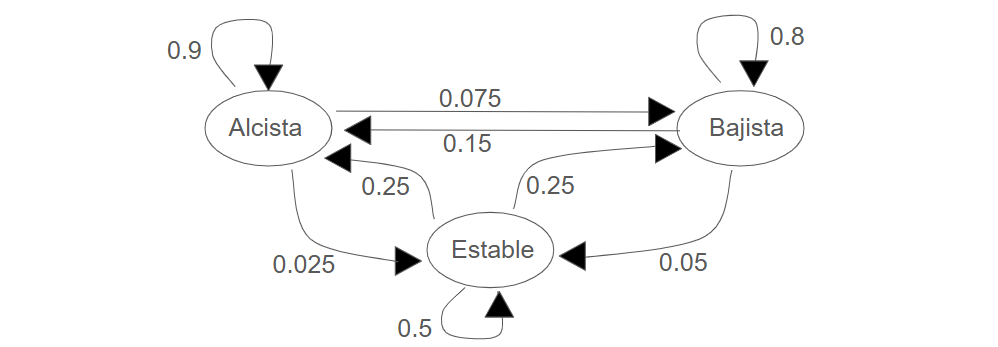
\includegraphics[width=0.8\textwidth]{../Images/Market/Market4.png}
}}
\only<5->{
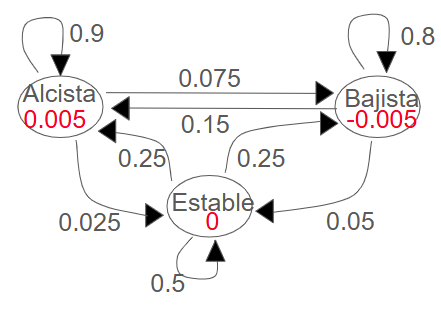
\includegraphics[width=0.45\textwidth]{../Images/Market/MarketWithReward.png}}
\end{center}
\begin{itemize}
\item<6-> Ganancia o pérdida dependiendo 
del estado
\item<7-> Interpretación: Inversión de \$1 resulta
en $\$(1+r(x))$ al final de una semana con estado $x$
\item<8-> $r(\mathbf{Alcista}) = 0.005, r(\mathbf{Bajista}) = -0.005,
r(\mathbf{Estable}) = 0$
\item<9-> Invirtiendo \$1 hoy, cuánta plata habrá 
después de 3 semanas?
\end{itemize}
\end{itemize}
\end{frame}

\begin{frame}{Proceso Markoviano con Recompensa}
Invirtiendo \$1 hoy, cuánta plata habrá después de 3 semanas?
\begin{itemize}
\item<2-> Consideramos la secuencia de estados $x_0,~x_1,~x_2$.
\begin{itemize}
\item<3-> La ganancia es 
\only<3-4>{
$$(1+r(x_0))(1+r(x_1))(1+r(x_2))-1$$
}
\only<5->
{$$
{\rm E}\left[(1+r(x_0))(1+r(x_1))(1+r(x_2)) | x_0 = x\right]-1
$$.}
\item<4-> En $t = 0$, no sabemos cuáles serán los próximos estados $x_1,~ x_2$. 
\only <5-> {Utilizamos el valor esperado!}
\item<6-> \textbf{Cómo calcularlo?}
\end{itemize}
\end{itemize}
\end{frame}

\begin{frame}{Una Aproximación}

$$
\begin{array}{l}
{\rm E}\left[ (1+r(x_0))(1+r(x_1))(1+r(x_2)) | x_0 = x\right]-1 \\
\mode<beamer>{\only<2>{=  {\rm E}\left[\sum\limits_{t=0}^2 r(x_t)|x_0 =x \right] + \\ {\rm E}\left[ \sum\limits_{t=0}^1\sum\limits_{\tau=t+1}^2 r(x_t)r(x_\tau)|x_0 = x\right] +  {\rm E}\left[ r(x_0)r(x_1)r(x_2)|x_0 = x\right] \\}}
\only<3>{=  {\rm E}\left[\sum\limits_{t=0}^2 r(x_t)|x_0 =x \right] +\\\underbrace{{\rm E}\left[ \sum\limits_{t=0}^1\sum\limits_{\tau=t+1}^2 r(x_t)r(x_\tau)|x_0 = x\right] +  {\rm E}\left[ r(x_0)r(x_1)r(x_2)|x_0 = x\right]}_{\approx 0}\\}
\visible<4->{ \approx  \textcolor{red}{{\rm E}\left[\sum\limits_{t=0}^2 r(x_t)|x_0 =x \right]}}
\end{array}
$$

\only<3>{Como r es pequeño, los productos r(x)r(y) son mucho menores que r(x), así que vamos a simplificar la expresión.}

\visible<5->{
\begin{itemize}
    \item Vamos a derivar un algoritmo para calcular el valor esperado. 
    \item También es posible trabajar con la expresión multiplicativa, pero la suma es más comúnmente utilizada.
\end{itemize}}
\end{frame}

\begin{frame}{Evaluando MRPs - Intuición}
\begin{itemize}
\item Cómo podríamos construir un jugador de ajedrez?
\begin{center}
 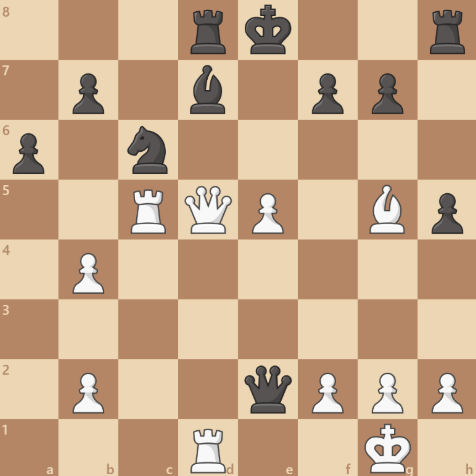
\includegraphics[width=0.5\textwidth]{../Images/Figures/Chess.png}   
\end{center}
\item<2-> Si tuviéramos una función para evaluar la probabilidad de ganar el juego a partir de cada posición, podríamos elegir la mejor acción
\item<3-> Esa función existe y es bien definida para MRPs y MDPs. Se denomina {\bf función valor.}
\end{itemize}
\end{frame}

\begin{frame}{Evaluando MRPs - Intuición}
\begin{itemize}
\item El concepto de función valor es central para la toma de decisiones secuenciales.
\item<2-> Otro concepto que vamos a utilizar es la idea de {\bf recursión}.
\item<3-> Para eso, vamos a representar el proceso con un nuevo grafo, utilizando el tiempo como segundo eje.
\end{itemize}
\begin{center}
\only<4>{
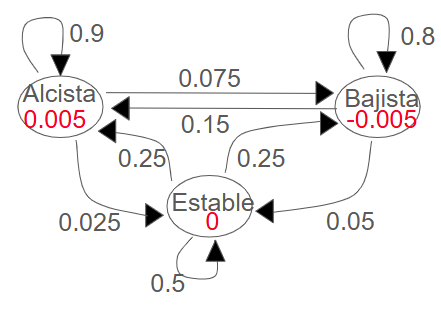
\includegraphics[width=0.8\textwidth]
{../Images/Market/MarketWithReward.png}}
\only<5>{
\hspace{-1.1cm}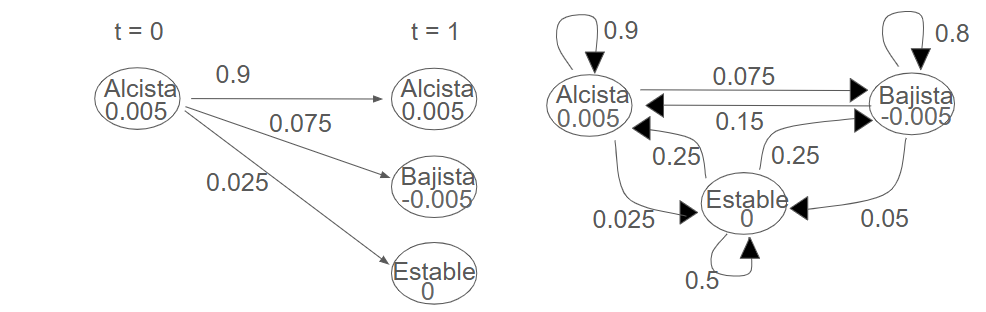
\includegraphics[width=1.1\textwidth]
{../Images/Market/Recursion1.png}}
\only<6>{
\hspace{-1.1cm}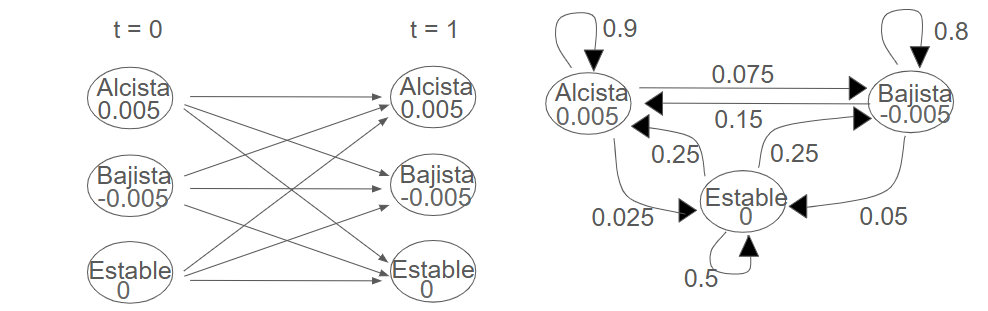
\includegraphics[width=1.1\textwidth]
{../Images/Market/Recursion2.png}}
\only<7->{
\hspace{-1cm}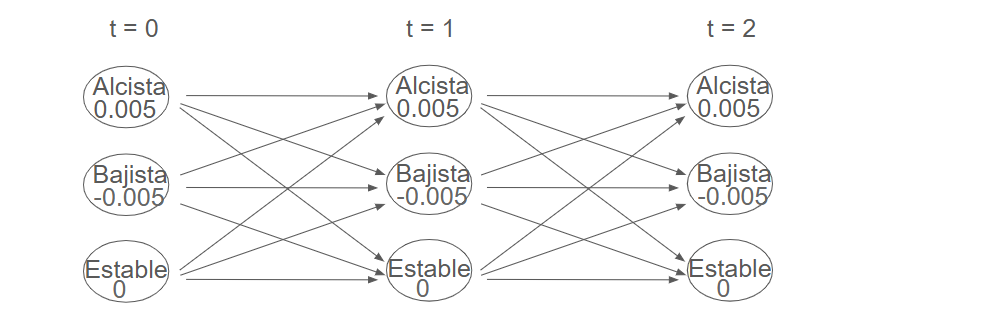
\includegraphics[width=1.1\textwidth]
{../Images/Market/Recursion3.png}}
\end{center}
\only<8->{\textcolor{red}{Idea: resolver una serie de problemas más fáciles, hasta llegar a la respuesta original.}}
\end{frame}

\begin{frame}{Calculando La Función Valor Por Recursión}
\begin{center}
\mode<beamer>{
\only<1-2>{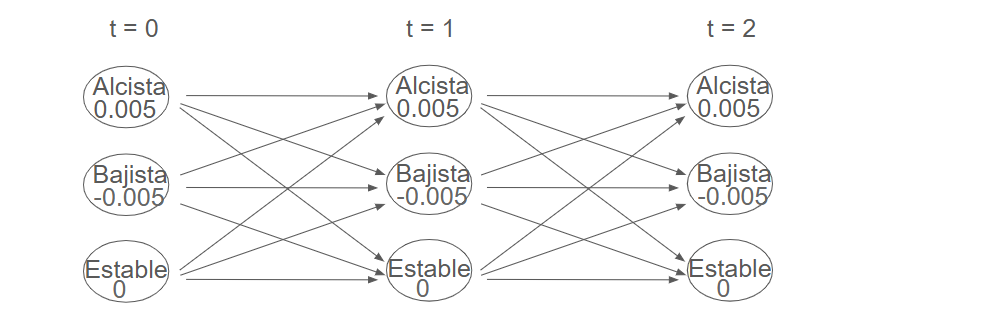
\includegraphics[width=0.8\textwidth]
{../Images/Market/Recursion3.png}}
\only<3-4>{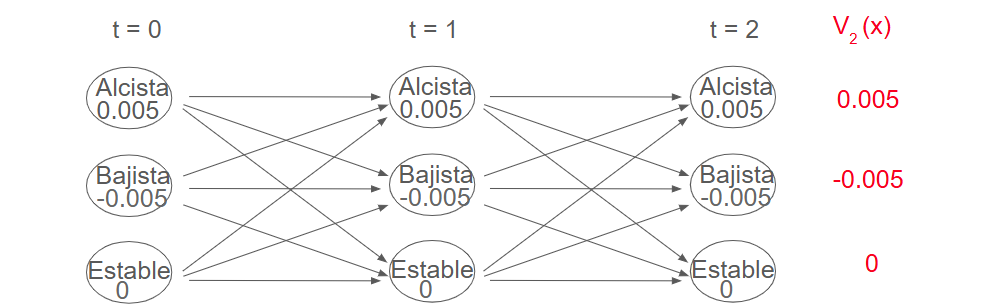
\includegraphics[width=0.8\textwidth]
{../Images/Market/Recursion4.png}}}
\only<5-7>{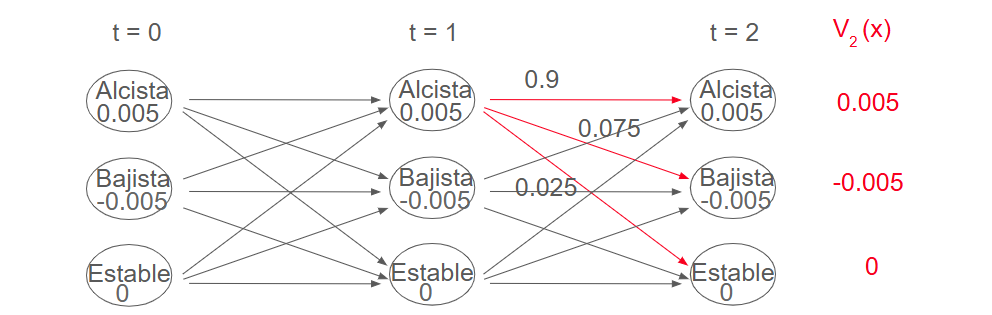
\includegraphics[width=0.8\textwidth]
{../Images/Market/Recursion5.png}}
\mode<beamer>{
\only<8>{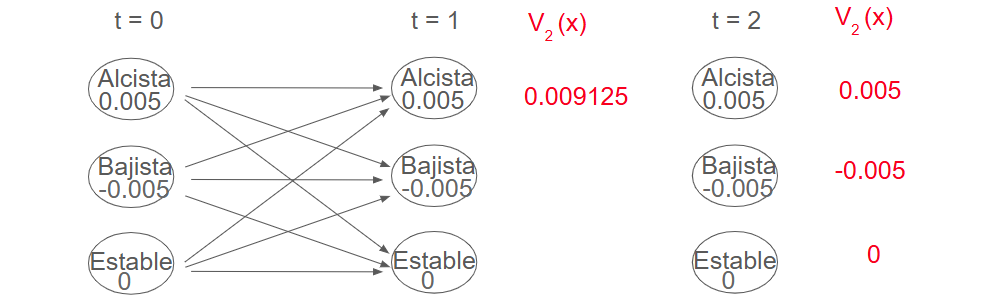
\includegraphics[width=0.8\textwidth]
{../Images/Market/Recursion6.png}}
\only<9-10>{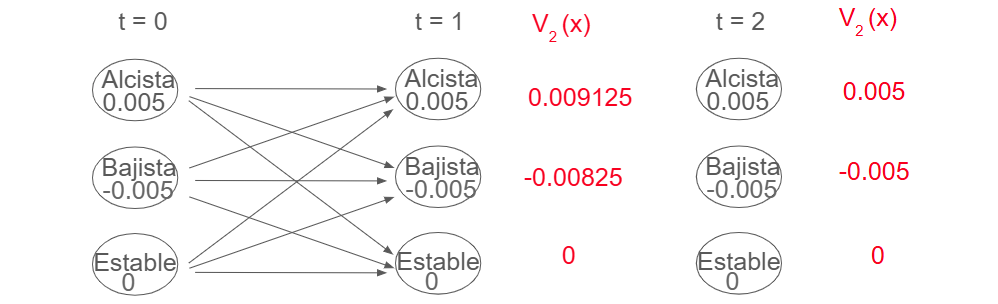
\includegraphics[width=0.8\textwidth]
{../Images/Market/Recursion7.png}}
\only<11->{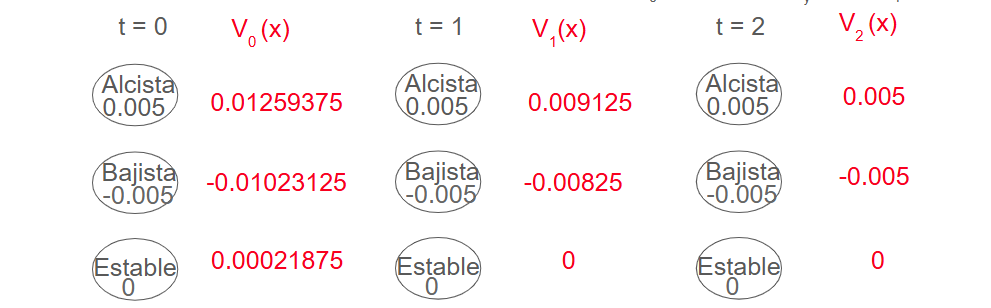
\includegraphics[width=0.8\textwidth]
{../Images/Market/Recursion8.png}}}
\end{center}
$V_t(x)$ = ganancia total esperada empezando en el estado $x$ en tiempo $t$.
\begin{enumerate}
\item<2->Calculamos $V_2(x) = r(x)$.
\item<4->Retrocedemos una semana y calculamos 
$V_1 (x)= r(x)+\sum_y P(x,y)V_2(y)$
\mode<beamer>{\only<5-9>{{\small
$$
\begin{array}{ccl}
V_1(\mathbf{A}) & = & r(\mathbf{A})+ \sum_y P(\mathbf{A},y) V_2(y)\\
\only<6-9> {& = & 0.005+0.9\times 0.005+0.075\times (-0.005)+0.025\times 0\\}
\only<7-9> {& = & 0.009125}
\end{array}
$$
}}

\only<9> {Repetimos el mismo procedimiento con $x=\mathbf{Bajista}$ y $x=\mathbf{Estable}$.}}
\item<10-> Retrocedemos otra semana y calculamos $V_0(x) = r(x) + \sum_yP(x,y)V_1(y).$
\end{enumerate}
\begin{itemize}
\item<12> \textcolor{red}{Invirtiendo \$1 at $t = 0$, si la semana actual es alcista se espera tener \$1.01259375 después de 3 semanas.}
\end{itemize}
\end{frame}

\begin{frame}{La Función Valor}
\begin{itemize}
\item Proceso markoviano con recompensa definido por la tupla $(S,P,r)$
\item<2-> Distintas maneras de combinar $r(x_t),~t=0,1,\dots$ en un único criterio (suma, multiplicación, medidas de riesgo)
\item<3->Una de las definiciones más comúnmente utilizadas es la recompensa total:
$$
V_t(x) = {\rm E}\left[\sum_{\tau=t}^T r(x_\tau)|x_t = x\right]$$
\begin{itemize}
\item $T$ es el \textbf{horizonte} (finito)
\end{itemize}
\end{itemize}
\end{frame}

\begin{frame}{La Función Valor}
\begin{itemize}
\item La función valor expresa la ganancia esperada, presente y futura, a partir del estado $x$
\item<2-> Si tenemos una evaluación de cada estado, la podemos utilizar para tomar decisiones
\item<3-> Por ejemplo, si tenemos dos aciones posibles en un estado $x$:
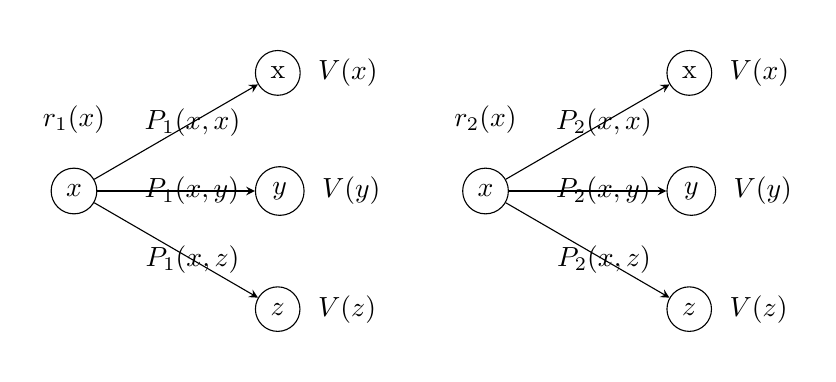
\begin{tikzpicture}[
    node distance=1.5cm and 2cm,
    every node/.style={draw, circle},
    >=stealth
  ]
  % Nodes
  \node (A) {$x$};
  \node[right=of A, yshift=1.5cm] (B) {x};
  \node[right=of A] (C) {$y$};
  \node[right=of A, yshift=-1.5cm] (D) {$z$};
\node (E)[right=of C] {$x$};
  \node[right=of E, yshift=1.5cm] (F) {x};
  \node[right=of E] (G) {$y$};
  \node[right=of E, yshift=-1.5cm] (H) {$z$};

  % Node labels
  \node[above=0.5pt of A, draw=none] {$r_1(x)$};
  \node[right=0.5pt of B, draw=none] {$V(x)$};
  \node[right=0.5pt of C, draw=none] {$V(y)$};
  \node[right=0.5pt of D, draw=none] {$V(z)$};
    \node[above=0.5pt of E, draw=none] {$r_2(x)$};
  \node[right=0.5pt of F, draw=none] {$V(x)$};
  \node[right=0.5pt of G, draw=none] {$V(y)$};
  \node[right=0.5pt of H, draw=none] {$V(z)$};

  % Arrows with labels
  \draw[->] (A) -- (B) node[pos=0.6, draw=none] {$P_1(x,x)$};
  \draw[->] (A) -- (C) node[pos=0.6, draw=none] {$P_1(x,y)$};
  \draw[->] (A) -- (D) node[pos=0.6,  draw=none] {$P_1(x,z)$};
    \draw[->] (E) -- (F) node[pos=0.6,  draw=none] {$P_2(x,x)$};
  \draw[->] (E) -- (G) node[pos=0.6,  draw=none] {$P_2(x,y)$};
  \draw[->] (E) -- (H) node[pos=0.6, draw=none] {$P_2(x,z)$};
\end{tikzpicture}
\item<4-> Podemos comparar $r_1(x)+\sum_{x'} P_1(x,x')V(x')$ y $r_2(x)+\sum_{x'} P_2(x,x')V(x')$ para decidir qué acción tomar.
\end{itemize}
\end{frame}

\begin{frame}{Factores de Descuento}
\begin{itemize}
\item Tenés dos opciones: ganar \$100 hoy, o ganar \$100 en un año. Es lo mismo?
\item<2-> Se puede expandir la definición introduciendo un factor de descuento: 
$$
V_t(x) = {\rm E}\left[\sum_{\tau=t}^T \alpha^{\tau-t}r(x_\tau)|x_t = x\right]
$$
\item<3-> Descontamos la recompensa $r(x_{\tau})$ en el periodo $\tau$ por $\alpha^{\tau-t}$
\begin{itemize}
\item<4-> Cuando más grande $\tau-t$, más grande el descuento
\end{itemize}
\item<5-> Interpretación económica (\$1 vale más en el presente que en el futuro) 
\item<6-> Menos confianza en lo que pasará en el futuro distante que cercano
\item<7-> $\alpha=0$ implica que el criterio de valoración es miope (solo la recompensa inmediata $r(x_t)$ es considerada)
\item<8-> $\alpha=1$ es equivalente a no tener un factor de descuento 
\end{itemize}
\end{frame}

\begin{frame}{Programación Dinámica}
\begin{itemize}
\item Definimos Vt(x) recursivamente:
{\small $$
\begin{array}{ccl}
V_T(x) & = & r(x) \\
V_t(x) & = & {\rm E}\left[\sum\limits_{\tau=t}^T \alpha^{\tau-t} r(x_\tau) | x_t = x\right] \\
\only<2->{& = & r(x) + \alpha {\rm E}\left[{\rm E} \left[\sum\limits_{\tau=t+1}^T \alpha^{\tau-(t+1)} r(x_\tau) | x_{t+1} = y\right] | x_t = x\right] \\}
\only<3->{& = & r(x) + \alpha \sum\limits_y P(x,y) V_{t+1}(y) }
\end{array}
$$}
\item<4-> Podemos usar notación de matrices para simplificar las ecuaciones:
$$
\begin{array}{ccl}
V_T &=& r \\
V_t & = & r+ \alpha P V_{t+1},~t = 0,...,T-1
\end{array}
$$
donde $r \in \Re^{|S|}$, $V_t \in \Re^{|S|}$, $P \in \Re^{|S|\times|S|}$.
\item<5-> Podemos implementar el algoritmo en Python.
\end{itemize}
\end{frame}

\begin{frame}{Observaciones}
\begin{itemize}
\item Asumimos que $r$ y $P$ no dependen de $t$, entonces el proceso markoviano es homogéneo en el tiempo. Pero se puede extender el resultado al caso en que dependen de $t$: 
$$
\begin{array}{ccl}
V_T &=& r_T \\
V_t & = & r_t+ \alpha P_t V_{t+1},~t = 0,...,T-1
\end{array}
$$
\item<2-> También asumimos que la recompensa es determinística, pero podemos incorporar casos en que es aleatoria:                $$
\bar{r}(x) = {\rm E}_w\left[r(x,w)\right]
$$                          
\item<3-> Si la recompensa depende del próximo estado además del actual, también se puede incorporar utilizando: 
$$
\bar{r}(x) = {\rm E}\left[r(x,x_{t+1})| x_t = x\right] = \sum_y P(x,y)r(x,y)
$$ 
\end{itemize}
\end{frame}

\begin{frame}{Procesos Markovianos de Decisión}
\begin{center}
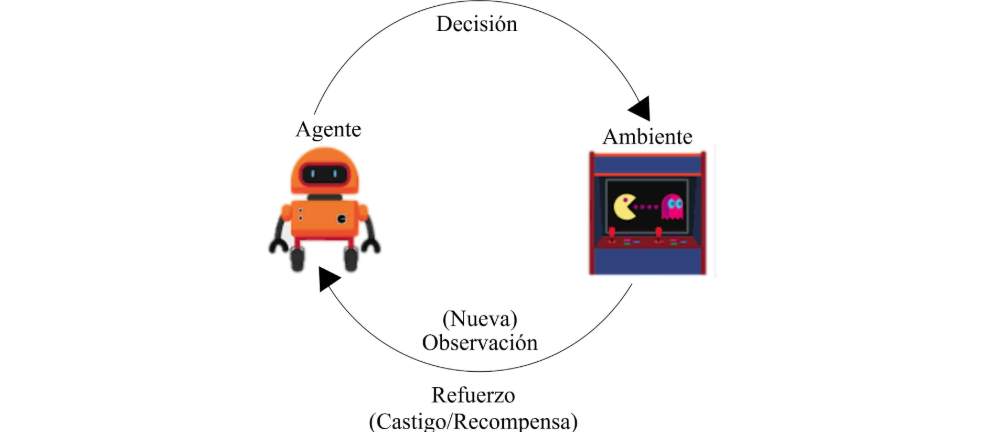
\includegraphics[width=0.8\textwidth]
{../Images/Figures/RL3.png}
\end{center}
\begin{itemize}
\item Hasta ahora, consideramos procesos markovianos $(S,P,r)$
\item<2-> Ahora agregaremos decisiones:
\begin{itemize}
\item<3-> Espacio de Estados $S$
\item<4-> Espacio de Acciones $A$
\item<5-> Recompensa $r_a(x)$ y probabilidad de transición $P_a(x,y)$
\begin{itemize}
\item Ahora dependen de la acción $a$ además del estado $x$
\end{itemize}
\end{itemize}
\item<6-> \textcolor{red}{Proceso Markoviano de Decisión caracterizado por la tupla $(S,A,P,r)$}
\end{itemize}
\end{frame}

\begin{frame}{Ejemplo: Precios Dinámicos}

Un vuelo tiene capacidad para 100 pasajeros. A cada día llega un posible pasajero que acepta pagar un precio máximo $m$ por el vuelo. Ese precio es desconocido a la aerolínea y distribuido con probabilidades {\small ${\rm Prob}(m = 50) = 1/2$, ${\rm Prob}(m = 70) = 1/3$, ${\rm Prob}(m = 120) = 1/6$.}

\vspace{0.5cm}
Qué precio la aerolínea debe ofrecer a cada día para maximizar su ganancia?
\end{frame}

\begin{frame}{Ejemplo: Precios Dinámicos - Modelo MDP - $(S,A,P,r)$}

Un vuelo tiene capacidad para 100 pasajeros. A cada día llega un posible pasajero que acepta pagar un precio máximo $m$ por el vuelo. Ese precio es desconocido a la aerolínea y distribuido con probabilidades {\small ${\rm Prob}(m = 50) = 1/2$, ${\rm Prob}(m = 70) = 1/3$, ${\rm Prob}(m = 120) = 1/6$.}
\begin{center}
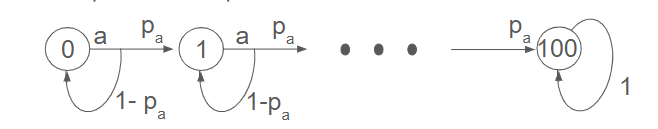
\includegraphics[width=0.9\textwidth]{../Images/Figures/Airline.png}
\visible<2->{
\begin{tabular}{|c|c|c|}
\hline
$a$ & $P_a(x,x+1) = {\rm Prob}(m\geq a) = p_a$ & $r_a(x) = a p_a$\\
\hline
50 & 1 & 50 \\
\hline
70 & 0.5 & 35 \\
\hline
120 & 1/6 & 20 \\
\hline
\end{tabular}}
\end{center}
\end{frame}

\begin{frame}{Ejemplo: Precios Dinámicos - Modelo MDP - $(S,A,P,r)$}

Un vuelo tiene capacidad para 100 pasajeros. A cada día llega un posible pasajero que acepta pagar un precio máximo $m$ por el vuelo. Ese precio es desconocido a la aerolínea y distribuido con probabilidades {\small ${\rm Prob}(m = 50) = 1/2$, ${\rm Prob}(m = 70) = 1/3$, ${\rm Prob}(m = 120) = 1/6$.}
\begin{itemize}
\item<2-> {\bf Espacio de estados}  
\only<4->{$S = \{0,1,\dots,100\}$}
\only<3->{
\begin{itemize}
\item Estado $x$ corresponde a la ocupación actual del avión, entonces $S = \{0,1,\dots,100\}$
\end{itemize}}
\item<5-> {\bf Espacio de acciones} \only<7->{$A = \{50, 70, 120\}$}
\begin{itemize}
\item<6-> Acción $a$ corresponde al precio cotizado cuando llega un posible pasajero, entonces $A = \{50, 70, 120\}$ 
\end{itemize}

\end{itemize}
\end{frame}

\begin{frame}{Ejemplo: Precios Dinámicos - Modelo MDP - $(S,A,P,r)$}

Un vuelo tiene capacidad para 100 pasajeros. A cada día llega un posible pasajero que acepta pagar un precio máximo $m$ por el vuelo. Ese precio es desconocido a la aerolínea y distribuido con probabilidades {\small ${\rm Prob}(m = 50) = 1/2$, ${\rm Prob}(m = 70) = 1/3$, ${\rm Prob}(m = 120) = 1/6$.}
\begin{itemize}
\item {\bf Matriz de transición} 
\begin{itemize}
\item<2-> Con el vuelo lleno (estado $x=100)$, asumiendo que no se permiten cancelaciones: $P_a(100,100) = 1$ (el vuelo se mantiene lleno)
\item<3-> Si $x<100$, si ofrecemos un asiento a precio $a$, el posible pasajero acepta ese precio si $m\geq a$. Entonces:
\end{itemize}
\only<4->{
$$\begin{array}{ccl}
P_a(x,x+1) & = & {\rm Prob}(m\geq a) \equiv p_a,~\forall x<100,~a \in A \\
P_a(x,x) & = & {\rm Prob}(m<a) \equiv 1-p_a,~\forall x<100,~a \in A  
\end{array}
$$}

\item<5-> {\bf Recompensa} 
\only<6->{
\begin{itemize}
\item Si el posible pasajero acepta el precio, recibimos $a$; si no acepta, no recibimos nada. Entonces:
\end{itemize}}
\only<7->{
$$
\begin{array}{ccl}
r_a(x) &=& a p_a,~\forall x=0,\dots,99,~a \in A\\
r_a(100) & = & 0,~\forall a \in A
\end{array}
$$}
\end{itemize}
\end{frame}



\begin{frame}{Políticas de Decisión}
\begin{itemize}
\item Dado un MDP, necesitamos determinar cómo tomar acciones. Estrategias especificando qué acción tomar son denominadas \textbf{políticas de decisión}.
\item<2-> Qué información debemos utilizar al tomar una acción?

Una opción son políticas que utilizan toda la información que tenemos hasta ese momento: $
a_t = u_t(x_0,a_0, r_0, x_1,a_1,r_1,...,x_{t-1},a_{t-1},r_{t-1},x_t)
$. 

Otro extremo serían políticas que no utilizan ninguna información: $a_t = u$.
\item<3-> Queremos encontrar políticas at que optimicen un criterio de optimalidad. Consideremos la recompensa total esperada: 
$$
\max_u {\rm E}\left[\sum_{t=0}^T r_{a_t}(x_t)\right]
$$
\item<4-> \textcolor{red}{Resulta que, para obtener optimalidad, es suficiente que la política dependa  solamente del estado actual: 
$$a_t = u_t(x_t)$$}
\end{itemize}
\end{frame}

\begin{frame}{Política Óptima}
\begin{itemize}
\item $u_t: S \mapsto A$ es una política indicando, para cada periodo $t$ y estado $x$, una acción $a = u_t(x)$.
\item<2-> Existe una política óptima $u^*$ que maximiza la suma esperada de recompensas.
\item<3-> Nuestro problema se vuelve:
\mode<beamer>{
$$
\only<3>{\max_u {\rm E}\left[\sum_{t=0}^T r_{u_t(x_t)}(x_t)\right]}
\only<4>{\max_u {\rm E}\left[\sum_{t=0}^T \underbrace{r_{u_t(x_t)}(x_t)}_{r_u(x_t)}\right]}
\only<5->{\max_u {\rm E}\left[\sum_{t=0}^T r_u(x_t)\right]}
$$}
\mode<handout>{
$$
\only<5->{\max_u {\rm E}\left[\sum_{t=0}^T r_u(x_t)\right]}
$$}
\item<6-> Considerando el horizonte $T$, el número de políticas posibles es $|A|^{|S|\times T}$
\begin{itemize}
\item<7-> Número de políticas crece exponencialmente con el número de estados y el horizonte
\end{itemize}
\item<8-> Pero podemos resolver el problema con más eficiencia…
\end{itemize}    
\end{frame}

\begin{frame}{Principio de Optimalidad}
\textbf{“Una política es óptima si, cualquiera sea el estado inicial y la primera acción tomada, las decisiones subsiguientes constituyen también una política óptima desde el nuevo estado.”}
— Richard Bellman
\begin{itemize}
\item<2-> Por ejemplo, si deseamos tomar el camino más corto entre puntos $A$ y $B$, y ese camino pasa por un punto $C$, entonces el subcamino entre $C$ y $B$ es el más corto entre eses dos puntos.
\item<3-> En general para MDPs, la política óptima empezando en el periodo $t+1$ es óptima también para el problema empezando en el periodo $t$, entonces se puede resolver por recursión, empezando por $t = T$ y retrocediendo hasta $t = 0$.
\end{itemize}
\end{frame}

\begin{frame}{Programación Dinámica Para MDPs}
\begin{enumerate}
\item En $t = T$, elegimos
$u^*_T(x) = \arg\max_{a \in A} r_a(x)$.
El valor de estar en un estado $x$ en $t = T$ es
$V_T^*(x) = \max_a r_a(x)$.
\item<2-> Si conocemos el valor óptimo para cada estado $x$ en el periodo $T+1$:
$V^*_{T+1}(x) = \max_u {\rm E}\left[\sum_{\tau=t+1}^T \alpha^{\tau-(t+1)}r_u(x_\tau) | x_{t+1} = t\right]$
podemos encontrar el valor y la política óptima en el periodo $t$
\visible<3->{
\begin{center}
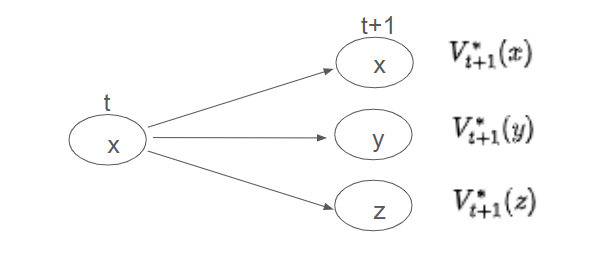
\includegraphics[width=0.6\textwidth]{../Images/Figures/Bellman.png}
\end{center}
}
\visible<4->{
Para cada acción a, recibimos:
$r_a(x)+\alpha \sum_y P_a(x,y) V_{t+1}^*(y)$
}
\visible<5->{
La mejor acción maximiza esa expresión. Entonces:
$$
\begin{array}{ccl}
V^*_t(x) & = & \max\limits_{a \in A} \left\{r_a(x)+\alpha \sum_y P_a(x,y) V_{t+1}^*(y)\right\} \\
u^*_t(x) & = & \arg\max\limits_{a \in A} \left\{r_a(x)+\alpha \sum_y P_a(x,y) V_{t+1}^*(y)\right\} 
\end{array}
$$
}
\end{enumerate}
\end{frame}

\begin{frame}{Programación Dinámica Para MDPs}
\begin{enumerate}
\item Hacemos $t = T$. Calculamos $$V_T^*(x) = \max_a r_a(x).$$
\item Hacemos $t = t-1$. Calculamos $$V^*_t(x) =  \max\limits_{a \in A} \left\{r_a(x)+\alpha \sum_y P_a(x,y) V_{t+1}^*(y)\right\}$$.
\item Si t = 0, fin. Si no, volvemos al paso 2.
\end{enumerate}
Derivamos la política óptima a partir de la función valor $V^*$:
$$
u^*_t(x) = \arg\max\limits_{a \in A} \left\{r_a(x)+\alpha \sum_y P_a(x,y) V_{t+1}^*(y)\right\} 
$$
\end{frame}

\begin{frame}{Ejemplo: Precios Dinámicos - Modelo MDP - $(S,A,P,r)$}

Un vuelo tiene capacidad para 100 pasajeros. A cada día llega un posible pasajero que acepta pagar un precio máximo $m$ por el vuelo. Ese precio es desconocido a la aerolínea y distribuido con probabilidades {\small ${\rm Prob}(m = 50) = 1/2$, ${\rm Prob}(m = 70) = 1/3$, ${\rm Prob}(m = 120) = 1/6$.}
\begin{center}
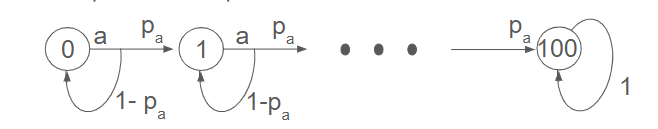
\includegraphics[width=0.9\textwidth]{../Images/Figures/Airline.png}
\begin{tabular}{|c|c|c|}
\hline
$a$ & $P_a(x,x+1)$ & $r_a(x)$\\
\hline
50 & 1 & 50 \\
\hline
70 & 0.5 & 35 \\
\hline
120 & 1/6 & 20 \\
\hline
\end{tabular}
\end{center}
Vamos a encontrar la política óptima con Python.
\end{frame}

\begin{frame}{Precios Dinámicos - Política Óptima}
\begin{center}
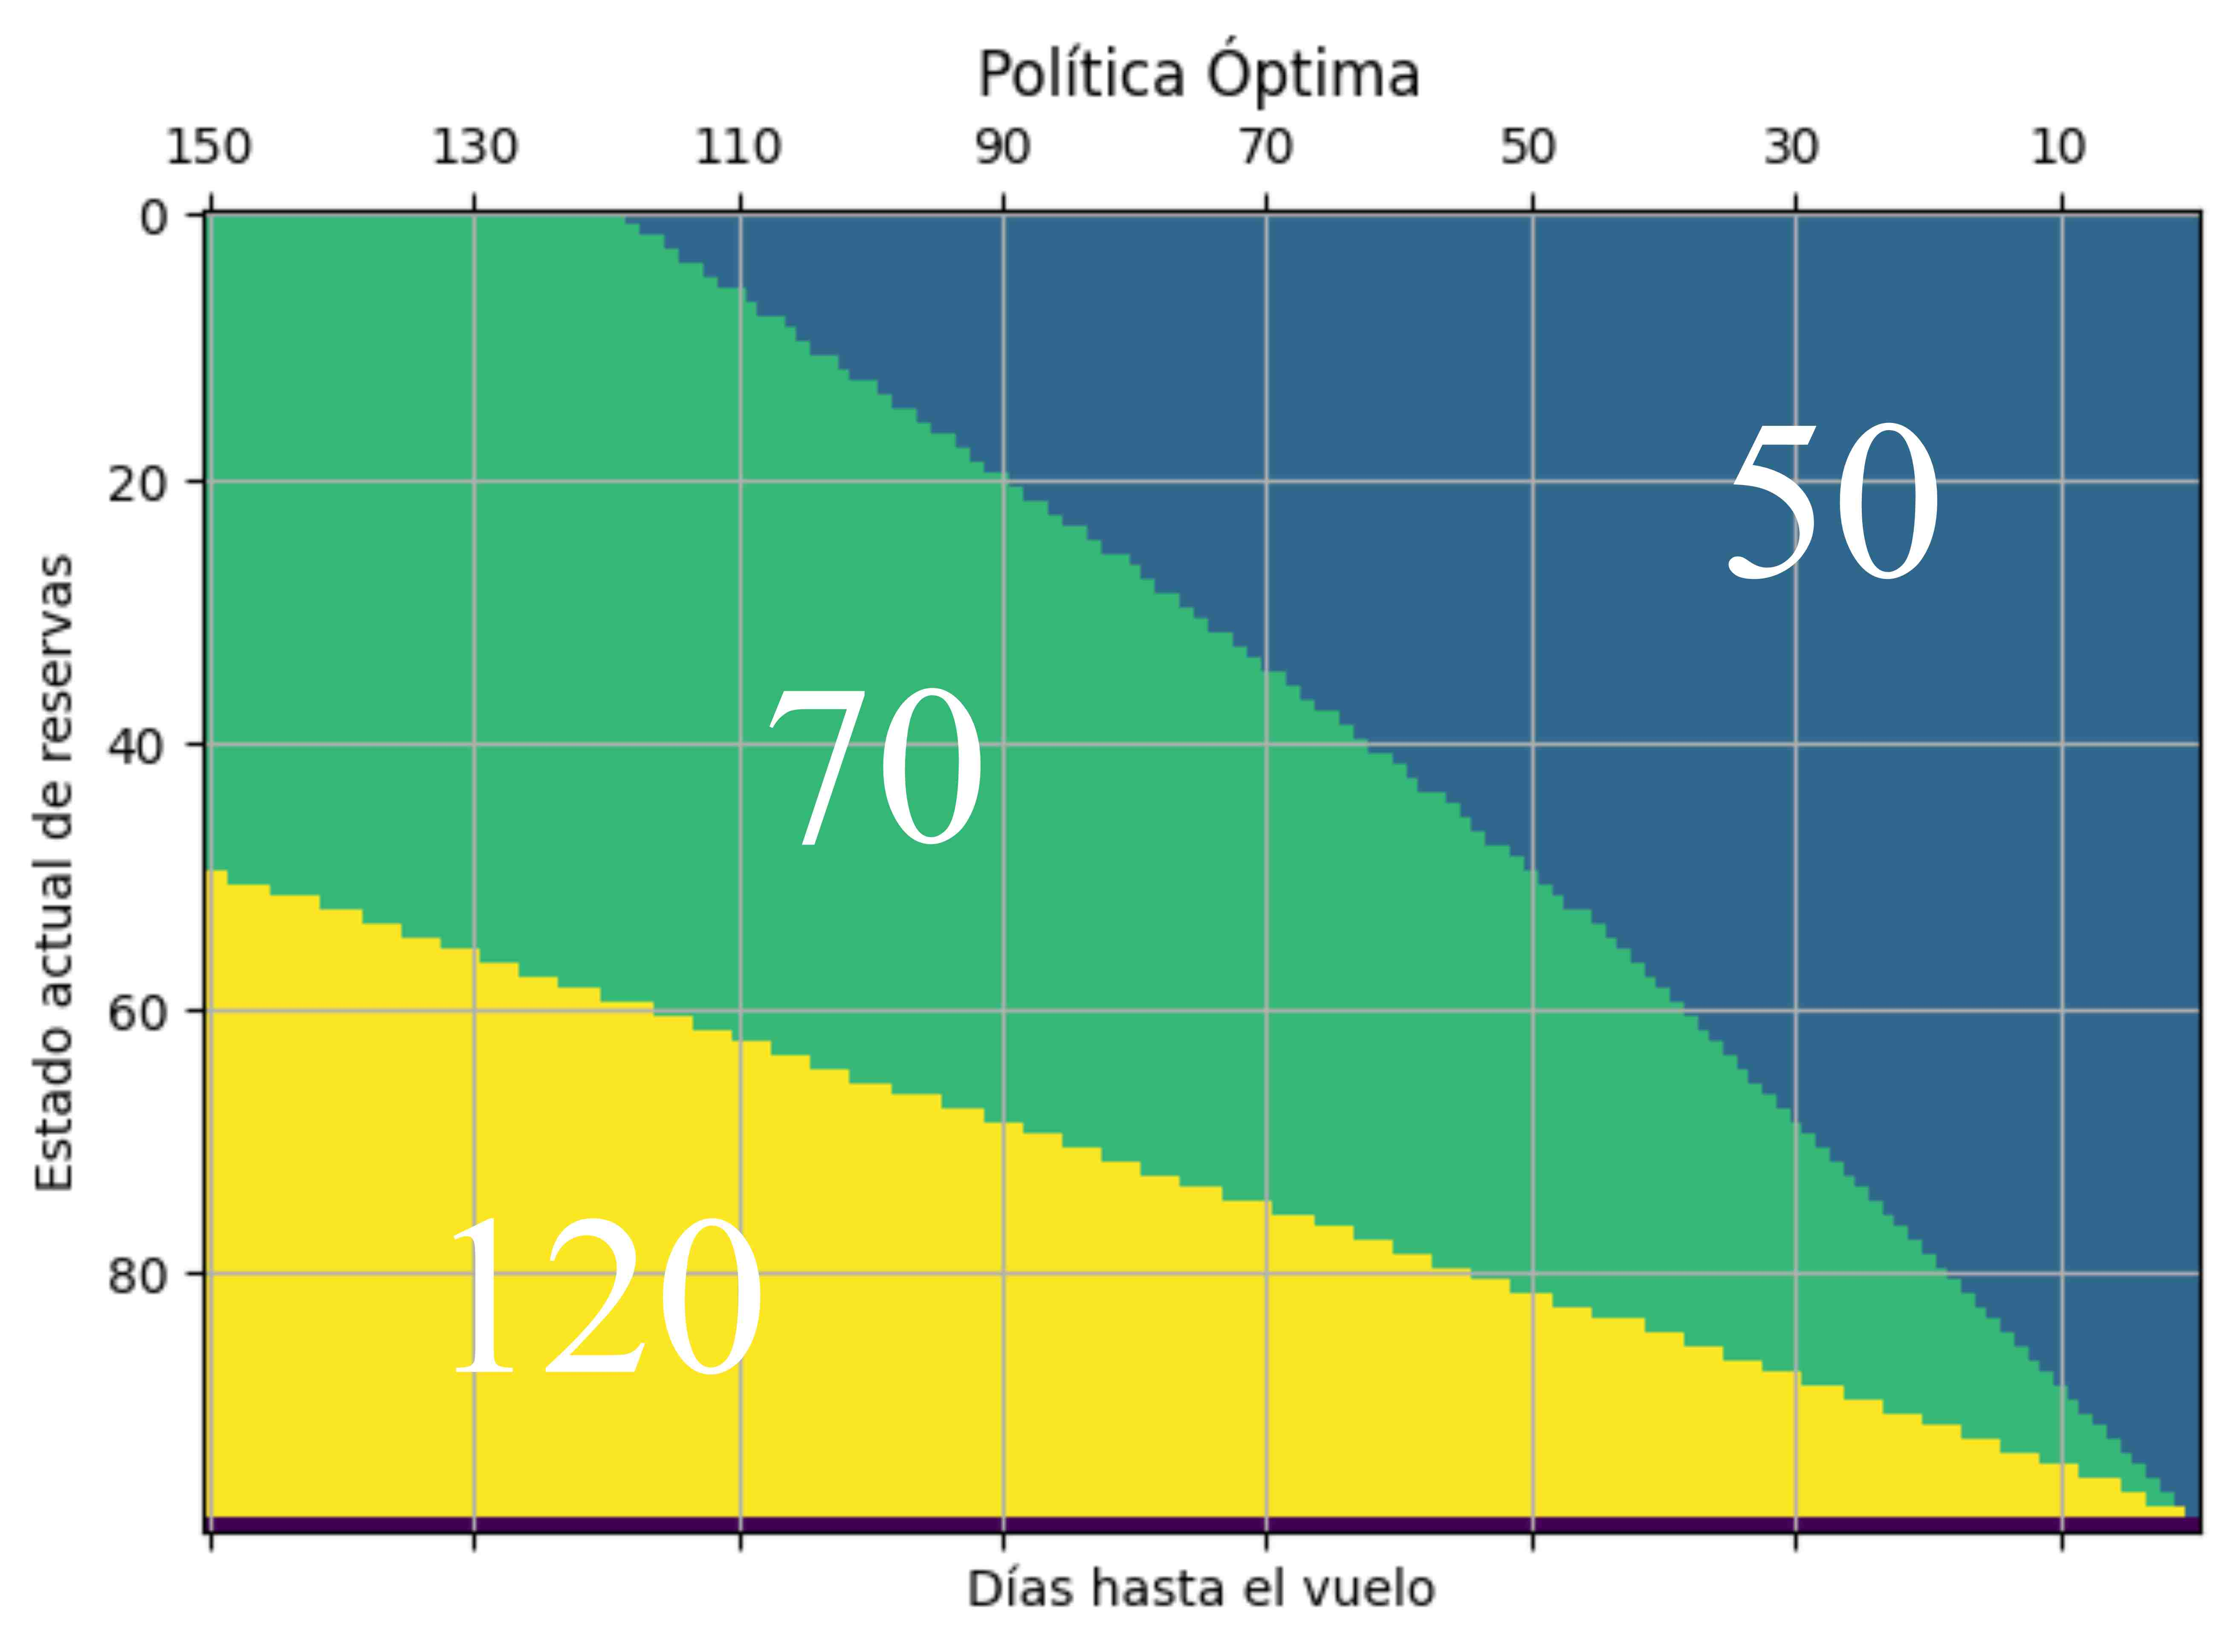
\includegraphics[width = 1\textwidth]{../Images/Figures/DynamicPrices.jpg}
\end{center}
\end{frame}

\begin{frame}{Precios Dinámicos - Ganancia}
\begin{center}
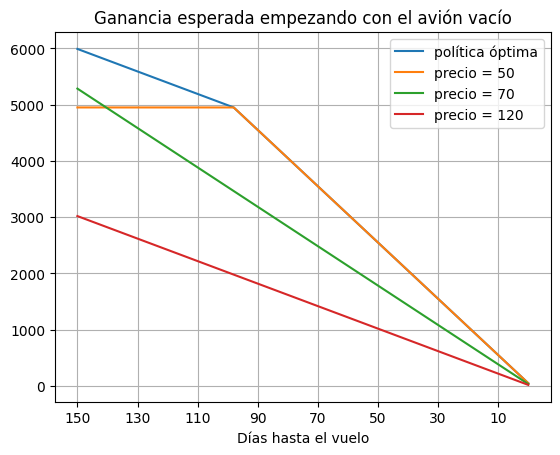
\includegraphics[width = 1\textwidth]{../Images/Figures/DynamicPricesValueAll.png}
\end{center}
\end{frame}

\begin{frame}{Estructura de Políticas}
\begin{itemize}
\item En el ejemplo anterior, la política óptima tiene una estructura intuitiva.
\item<2-> En otras aplicaciones, también se espera que la política óptima tenga ciertas características.
\begin{itemize}
\item<3-> Gestión de inventarios: comprar más mercadería basándose en límites.
\item<4-> Navegación: objectivos pueden ser equivalentes a buscar el camino más corto.
\end{itemize}
\item<4-> En situaciones prácticas, a veces es preferible una política con estructura interpretable a una más compleja.
\item<5-> En situaciones de aprendizaje por refuerzo, se puede directamente reducir la búsqueda a políticas con ciertas estructuras.
\end{itemize}    
\end{frame}

\begin{frame}{Diseño de La Función de Recompensa}
\begin{itemize}
\item Gestión de inventario (maximizar ganancia)
\only<2->{
\begin{center}
$r(x,a) = {\rm E}[\alpha \min(d,x+a) - \beta (x+a)]$
\end{center}
donde el estado $x$  es el nivel $x$ de inventario, la acción $a$ define cuánto aumentar el inventario, y $d$ es una variable aleatoria representando la demanda.}
\item<3-> Navegación (tiempo a destino)
\visible<4->{
\vspace{-0.1cm}
\begin{center}
$r(x) = \begin{cases} 
1 & {\rm if ~ x \neq x^*} \\
0 & {\rm if ~x = x^*}
\end{cases}
$
\end{center}

donde el estado $x$ es la posición y $x^*$ es la posición final.}
\item<5-> Juego de ajedrez
\visible<6->{
\vspace{-0.2cm}
$$
r(x) = \begin{cases} 
1 & {\rm if ~ x \in A} \\
-1 & {\rm if ~ x \in B} \\
0 & {\rm if ~ x \notin A\cup B} \\
\end{cases}
$$
donde el estado $x$ es la configuración del tableros y $A$, $B$ son los conjuntos de configuraciones donde el jugador gana y pierde, respectivamente.}
\end{itemize}  
\end{frame}

\begin{frame}{Diseño de La Función de Recompensa: }
\begin{itemize}
\item  En algunas situaciones, es necesario combinar varios criterios en una función de recompensa
\begin{itemize}
\item<2-> Gestión de usina eólica con backup de gas natural
\only<3->{
$$
r(x) = {\rm E}[\alpha x + \beta \max(d-x,0)]
$$
donde el estado $x$ es la potencia siendo proporcionada por gás y $d$ es una variable aleatoria indicando la demanda no atendida por energia eólica.}
\end{itemize}
\item<4-> En situaciones de aprendizaje por refuerzo, más consideraciones son necesarias al diseñar la función de recompensa
\begin{itemize}
\item<5-> la función puede ayudar o dificultar el aprendizaje (por ejemplo, funciones esparsas son difíciles de entrenar)
\item<6-> se puede deducir la función de recompensa a partir de un agente humano con buen desempeño (aprendizaje por refuerzo inverso)
\begin{itemize}
\item<6-> Pero también es posible que humanos implícitamente utilicen funciones de recompensa subóptimas (ejemplo: AlphaGo)
\end{itemize}
\end{itemize}
\end{itemize}
\end{frame}
\end{document}
